% *******************************************************************************
% * Copyright (c) 2007 by Elexis
% * All rights reserved. This document and the accompanying materials
% * are made available under the terms of the Eclipse Public License v1.0
% * which accompanies this distribution, and is available at
% * http://www.eclipse.org/legal/epl-v10.html
% *
% *  $Id: trustx.tex 2933 2007-07-29 10:05:35Z rgw_ch $
% *******************************************************************************
% !Mode:: "TeX:UTF-8" (encoding info for WinEdt)

\section{Elexis-TrustX-Embed }
\label{trustx}
Mit diesem Plugin können Arztrechnungen direkt an ein TrustCenter übermittelt werden, das Daten gem. TrustX-Standard austauscht (das sind sämtliche zur Zeit in der Schweiz operierende TrustCenter). Dieses Plugin funktioniert zur Zeit nur unter Windows.

Dieses Plugin fällt etwas aus dem Rahmen des Elexis-Konzepts, weil es verschiedene Abhängigkeiten von ClosedSource-Software hat und deswegen nicht auf allen unterstützten Betriebssystemen lauffähig ist. Leider lassen sich diese Abhängigkeiten zur Zeit noch nicht vermeiden, da das TrustX-System einerseits selbst auf geheimgehaltenen Quellen basiert und andererseits auf ASAS zurückgreift, welches seinerseits eine ClosedSource-Variante eines Public-Key-Tunnels ist.
Wenn Sie möchten, dass diese Situation sich ändert, dann fragen Sie als TC-Kunde und als ASAS-Kunde nach OpenSource-Implementationen der Schnittstellen für den Datentransfer (es gibt keine sachlichen Gründe dagegen; gute Verschlüsselung basiert nie auf Geheimhaltung der Quellen, sondern auf der Stärke des Algorithmus).
Nach dieser Vorbemerkung nun zu den angesprochenen Bedingungen.

\subsection{Voraussetzungen}
Sie benötigen Elexis auf einem Windows-Computer. In Elexis muss das Plugin elexis-arzttarife-schweiz  enthalten sein (ist standardmässig immer der Fall). Ausserdem benötigen Sie einen \href{http://www.hin.ch}{HIN-Account} und den \href{http://www.hin.ch/asas}{ASAS-Client}. Schliesslich muss auch noch der \href{http://www.trustx.ch/trustx-praxis/documents/setup-2_1_14.exe}{TrustX-Client} installiert sein. Der ASAS-Client und der TrustX-Client müssen korrekt konfiguriert sein.

\subsection{Installation}
Es genügt, das \href{http://www.elexis.ch/files/elexis-trustx-embed.zip}{elexis-trustx-embed- Plugin} herunterzuladen und im Elexis-Verzeichnis zu entpacken. Nach dem nächsten Start von Elexis steht es zur Verfügung.

\subsection{Funktionsweise}
\begin{wrapfigure}{l}{6cm}
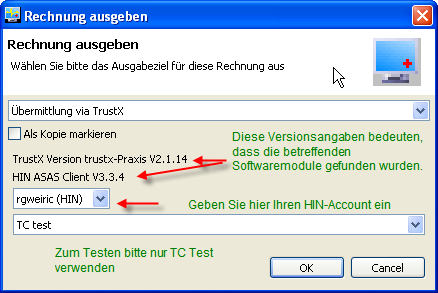
\includegraphics[width=6cm]{images/trustx.png}
\caption{TrustX-Transfer}
\label{fig:trustx}
\end{wrapfigure}
% trustx.png: 438x293 pixel, 96dpi, 11.59x7.75 cm, bb=0 0 328 220

Trustx-embed klinkt sich in das Rechnungsaus\-gabe-System ein. Sie können beim Ausgeben einer Rechnung als Ausgabeziel einfach statt einem Drucker die Option \textit{Übermittlung via Trustx} angeben, dann erscheint ein Dialog wie in Abb. \ref{fig:trustx}:

Achten Sie darauf, ob TrustX und ASAS korrekt gefunden wurden, und wählen Sie den richtigen Account und das richtige TrustCenter aus. Nach Klick auf OK werden die gewählten Rechnungen durch den verschlüsselnden ASAS-Tunnel gesichert an dieses Trust-Center übermittelt.

\subsection{Rückweisungen}
Vor allem am Anfang wird es Ihnen öfters passieren, dass Rechnungen vom TrustCenter zurückgewiesen werden. Mal fehlt der Kostenträger, mal ist eine EAN einer der beteiligten Stellen nicht korrekt angegeben etc. Alles Dinge, die bei Rechnungen auf Papier nicht so ins Gewicht fielen. Alle Zurückgewiesenen Rechnungen erhalten den Status \textit{fehlerhaft} und können so in der Rechnungen-View aufgefunden und korrigiert werden.

Achten Sie vor dem Übermitteln von Rechnungen auf folgende Punkte:
\begin{itemize}
 \item Jede Rechnung muss einem Fall zugeordnet sein, welcher
\begin{itemize}
 \item einen Garanten und einen Kostenträger hat
\item Einen Mandanten hat
\end{itemize}
\item Jede Rechnung muss mindestens eine Diagnose oder einen Diagnosecode haben. Das ist dann der Fall, wenn bei mindestens einer der verrechneten Konsultationen mindestens eine Diagnose angegeben wurde.
\item Der Mandant muss eine korrekte EAN haben (einzugeben z.B. in der Perspektive  \textit{Kontakte}). Sie können Ihre EAN bei der FMH erfragen, falls noch nicht bekannt.
\item Der Kostenträger muss eine korrekte EAN haben (einzugeben z.B. in der Perspektive \textit{Kontakte}). Sie können die EAN der Krankenversicherer jeweils direkt bei diesen erfragen, oder auch auf einer der im Internet verfügbaren Listen nachschlagen, z.B. bei der \href{http://www.sgim.ch/info/tarmed/EAN_KV.pdf}{SGIM}.

\end{itemize}

\textit{Die Entwicklung dieses Plugins wurde von Dr. med. S. Henzi,
Bern finanziert, der es allen anderen Elexis-Anwendern
kostenlos zur Verfügung stellt.}


